\documentclass[12pt,addpoints]{repaso}
\grado{3}
\nivel{Secundaria}
\cicloescolar{2024-2025}
\materia{Matemáticas}
\unidad{2}
\title{Practica la Unidad}
\aprendizajes{\footnotesize%
\item Usa e interpreta las medidas de tendencia central (moda, media aritmética y mediana) y el rango
de un conjunto de datos, y decide cuál de ellas conviene más en el análisis de los datos en cuestión
    \item Formula expresiones de primer grado para representar propiedades
    (perímetros y áreas) de figuras geométricas y verifica equivalencia de expresiones, tanto
    algebraica como geométricamente (análisis de las figuras).
    \item Resuelve problemas mediante la formulación y solución algebraica de ecuaciones lineales.
    \item Calcula el área y volumen de piramides, prismas y cilindros rectos.
    }
\author{Melchor Pinto, J.C.}
\begin{document}
\INFO%
\begin{questions}
    \section*{Probabilidad y estadística}
    \subsection*{Media, Mediana, Moda y Desviación media}
    \questionboxed[4]{Determina la mediana y la moda en los siguientes conjuntos de datos:
        \begin{multicols}{2}
            \begin{parts}
                \part 80, 82, 85, 88, 90, 88, 91, 85, 95, 88, 88, 97, 100. \\[1em]
                La media es: \fillin[$89$][0.4in]. \\
                La mediana es: \fillin[$88$][0.4in].\\
                La moda es: \fillin[$88$][0.4in].  \\

                \part Los puntajes obtenidos en un juego son: 54, 55, 59, 61, 77, 58, 55, 71, 59, 55, 60, 53, 56 y 60 puntos. \\[1em]
                La media es: \fillin[$59.5$][0.4in]. \\
                La mediana es: \fillin[$58.5$][0.4in].\\
                La moda es: \fillin[$55$][0.4in]. \\
                La desviación media es: \fillin[$4.5$][0.4in].

                \part 22, 25, 21, 23, 29, 30, 28, 27, 23, 26. \\[1em]
                La media es: \fillin[$25.4$][0.4in]. \\
                La mediana es: \fillin[$25.5$][0.4in].\\
                La moda es: \fillin[$23$][0.4in].\\
                La desviación media es: \fillin[$2.6$][0.4in].

                \part Las estaturas de un grupo de personas son: 170, 168, 169, 171, 168, 172, 168, 171 y 173 cm. \\[1em]
                La media es: \fillin[$170$][0.4in]. \\
                La mediana es: \fillin[$170$][0.4in].\\
                La moda es: \fillin[$168$][0.4in]. \\
            \end{parts}
        \end{multicols}
    }


    \subsection*{Eventos mutuamente excluyentes}
    \questionboxed[3]{Resuelve los siguientes problemas:
        \begin{multicols}{3}

            \begin{parts}\footnotesize%
                \part En una urna hay 10 pelotas azules, 5 verdes, 15 blancas y 20 negras. Calcula la probabilidad de sacar una pelota negra.

                \begin{solutionbox}{2cm}
                \end{solutionbox}

                \part Si se lanzan tres monedas al aire, calcula la probabilidad de que caiga puro sol.

                \begin{solutionbox}{2cm}
                \end{solutionbox}

                \part En una urna hay 8 pelotas moradas, 12 naranjas, 7 rojas, 11 azules y 7 blancas. Calcula la probabilidad de sacar una pelota negra.

                \begin{solutionbox}{2cm}
                \end{solutionbox}
            \end{parts}
        \end{multicols}

    }

    \section*{ Figuras y cuerpos geométricos}

    \subsection*{Perímetro y Área}
    \questionboxed[3]{Encuentra el perímetro y el área de las siguientes figuras:
        \begin{multicols}{3}
            \begin{parts}
                % \part 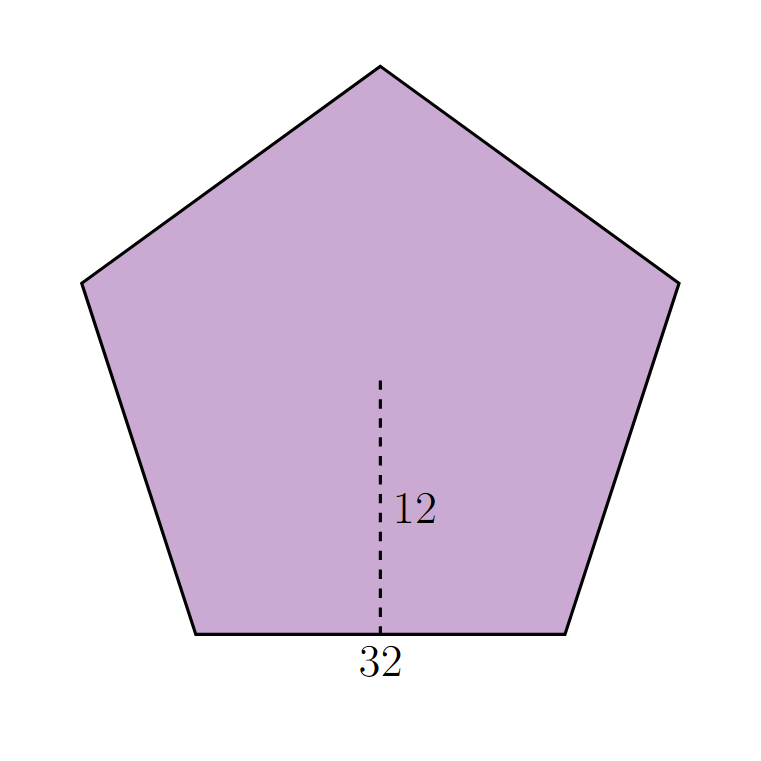
\includegraphics[width=\linewidth]{mex_0018.png}
                % Perímetro: \fillin[$$ u][0.4in] \hfill Área: \fillin[$$ u$^2$][0.4in]

                % \part 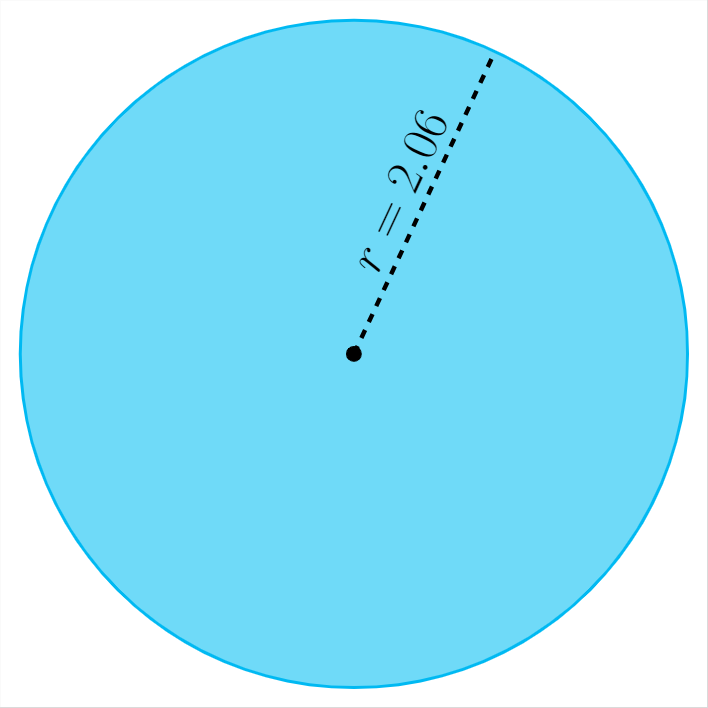
\includegraphics[width=\linewidth]{mex_0001.png}
                % Perímetro: \fillin[$$ u][0.4in] \hfill Área: \fillin[$$ u$^2$][0.4in]

                % \part 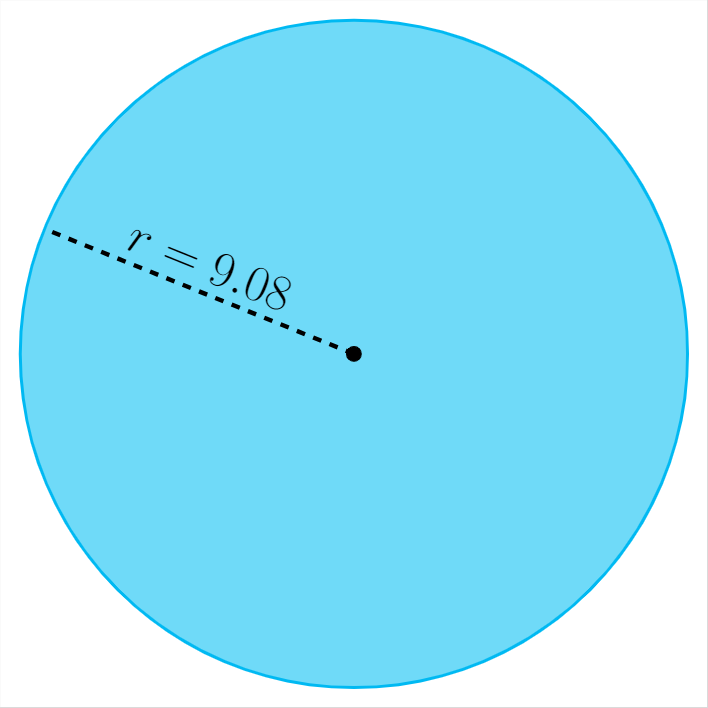
\includegraphics[width=\linewidth]{mex_0012.png}
                % Perímetro: \fillin[$$ u][0.4in] \hfill Área: \fillin[$$ u$^2$][0.4in]

                \part 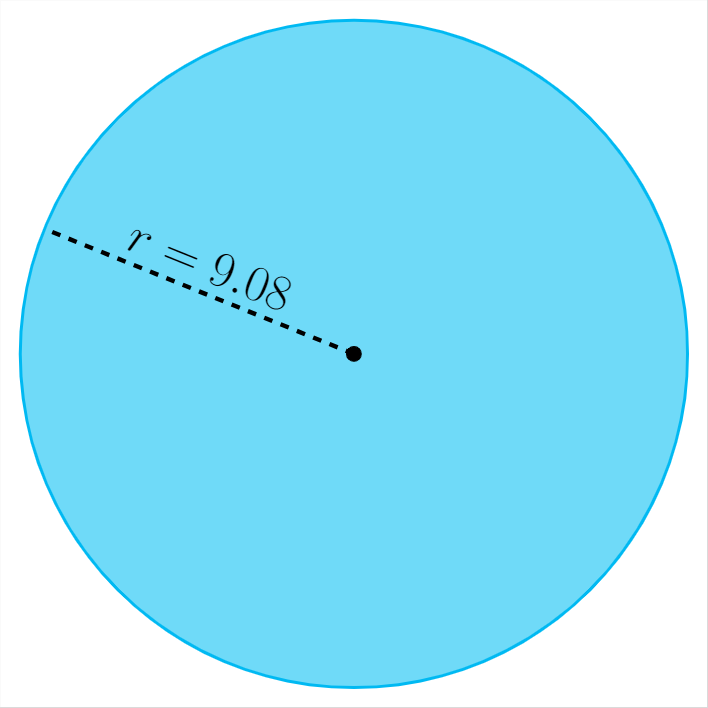
\includegraphics[width=0.8\linewidth]{mex_0013.png}
                Perímetro: \fillin[$$ u][0.4in] \hfill Área: \fillin[$$ u$^2$][0.4in]

                \part 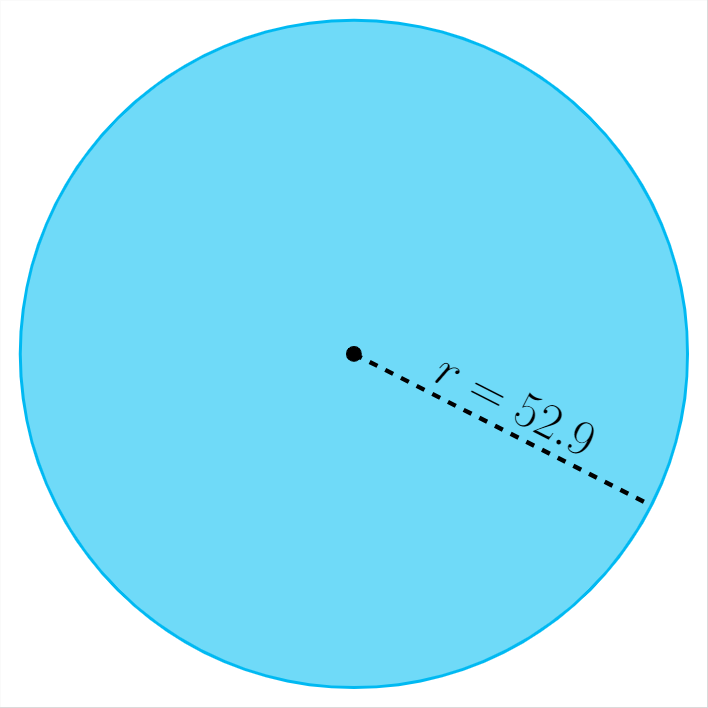
\includegraphics[width=0.8\linewidth]{mex_0004.png}
                Perímetro: \fillin[$$ u][0.4in] \hfill Área: \fillin[$$ u$^2$][0.4in]

                % \part 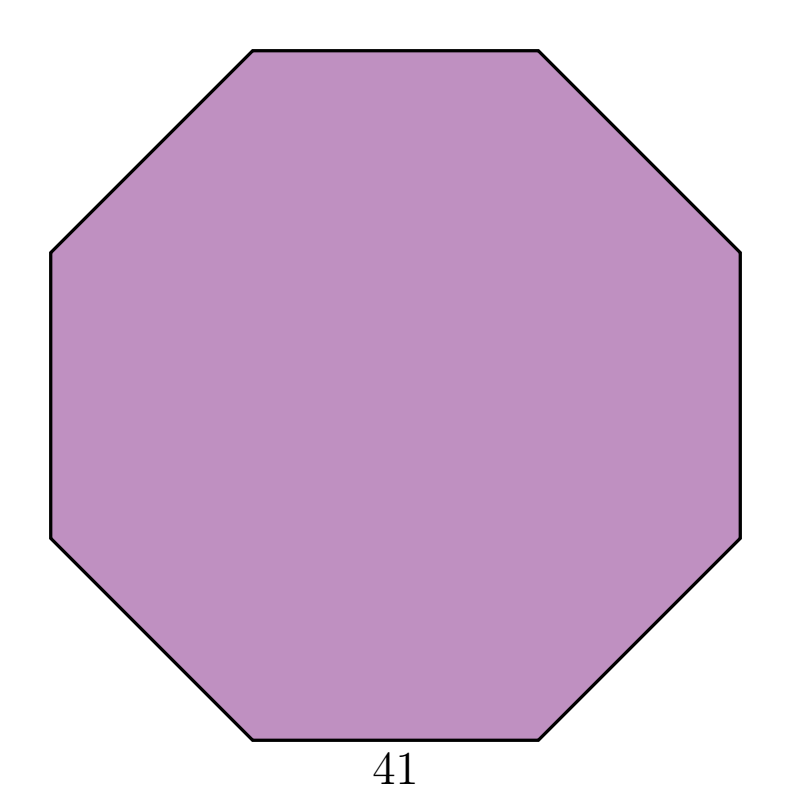
\includegraphics[width=\linewidth]{mex_0005.png}
                % Perímetro: \fillin[$$ u][0.4in] \hfill Área: \fillin[$$ u$^2$][0.4in]

                % \part 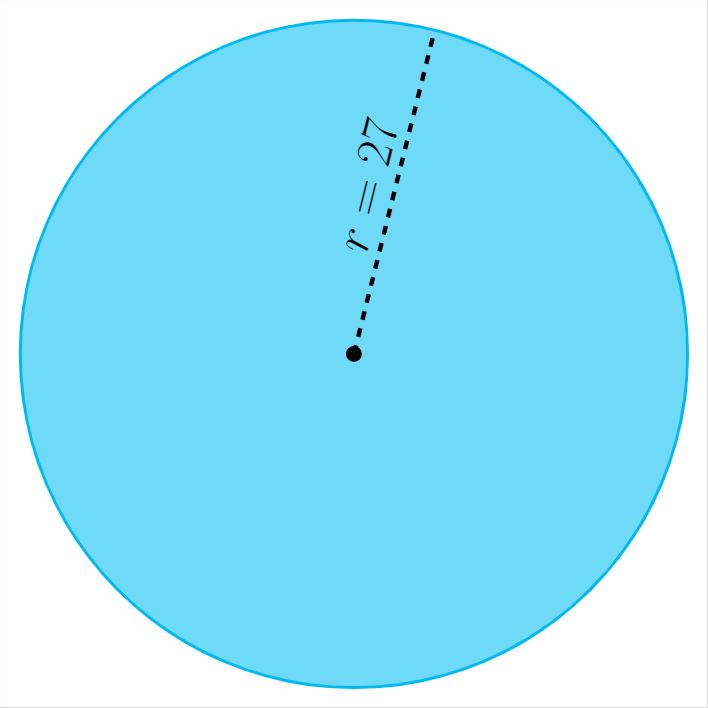
\includegraphics[width=\linewidth]{mex_0006.png}
                % Perímetro: \fillin[$$ u][0.4in] \hfill Área: \fillin[$$ u$^2$][0.4in]

                % \part 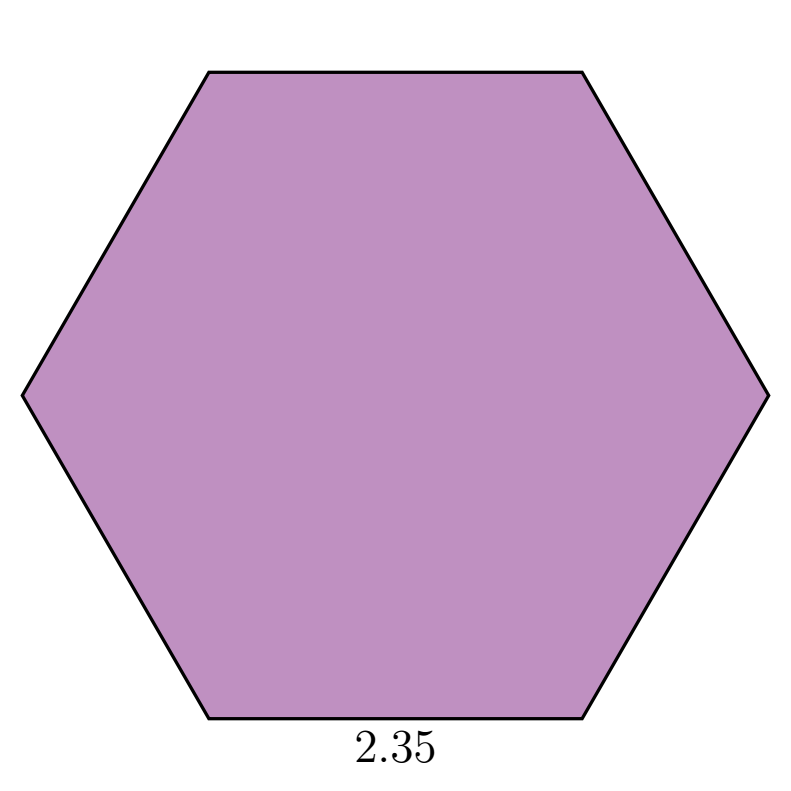
\includegraphics[width=\linewidth]{mex_0007.png}
                % Perímetro: \fillin[$$ u][0.4in] \hfill Área: \fillin[$$ u$^2$][0.4in]

                \part 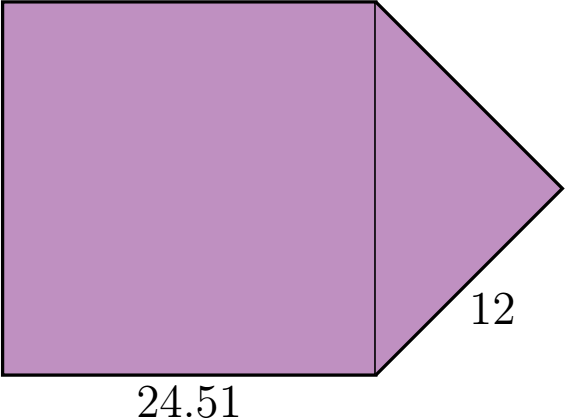
\includegraphics[width=0.8\linewidth]{mex_0014.png}
                Perímetro: \fillin[$$ u][0.4in] \hfill Área: \fillin[$$ u$^2$][0.4in]

            \end{parts}
        \end{multicols}
    }

    \subsection*{Resolución de problemas}
    \questionboxed[4]{Resuelve los siguientes problemas:
        \begin{multicols}{2}
            \begin{parts}\footnotesize%
                \part Calcula la altura de un prisma que tiene como área de la base 6 m$^2$ y 66 m$^3$ de capacidad.

                \begin{solutionbox}{1cm}
                \end{solutionbox}

                \part Calcula la altura de un prisma que tiene como área de la base 8 m$^2$ y 120 m$^3$ de capacidad.

                \begin{solutionbox}{1cm}
                \end{solutionbox}

                \part Ricardo quiere poner una barda alrededor de un terreno pentagonal que mide 15 metros por lado. ¿Cuánta barda necesitará Ricardo para poner barda en todo el terreno?

                \begin{solutionbox}{1cm}
                \end{solutionbox}

                \part ¿Cuál es el perímetro de un campo de fútbol que mide 95.12 metros de largo y 45.27 metros de ancho?

                \begin{solutionbox}{1cm}
                \end{solutionbox}
            \end{parts}
        \end{multicols}
    }

    \subsection*{Área lateral, Área total y Volumen}
    \questionboxed[4]{Calcula el volumen, el área lateral y el área total de las siguientes figuras:
        \begin{multicols}{2}
            \begin{parts}
                \part 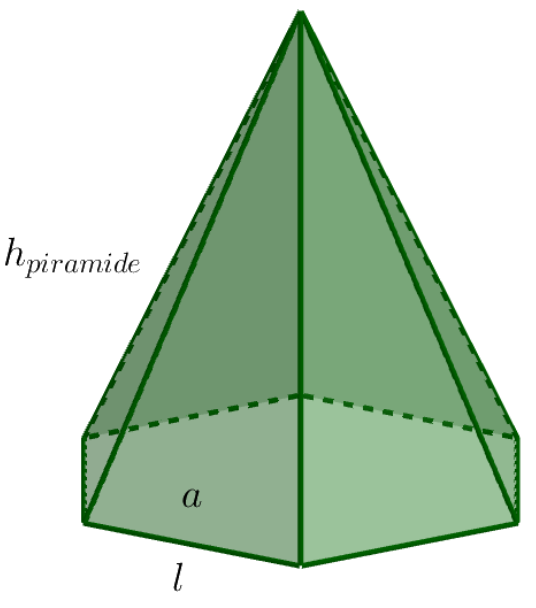
\includegraphics[width=0.8\linewidth]{mex_0022.png}
                Prisma cuyos lados "l" de la base miden 8 cm y la altura "h" mide 21 cm.\\
                Volumen: \fillin[$$ u$^3$][0.4in] \\A. Lateral: \fillin[$$ u][0.4in] \\ A. Total: \fillin[$$ u$^2$][0.4in]

                % \part 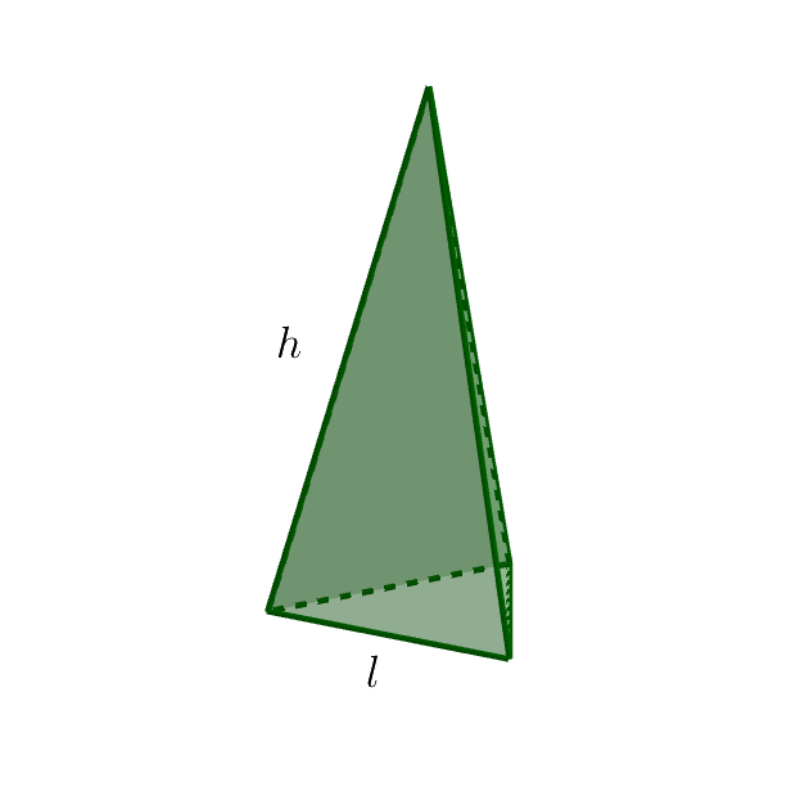
\includegraphics[width=\linewidth]{mex_0023.png}
                % Pirámide cuyos lados "l" de la base miden 13 cm y la altura "h" mide 42 cm.\\
                % Volumen: \fillin[$$ u$^3$][0.4in] \\A. Lateral: \fillin[$$ u][0.4in] \\ A. Total: \fillin[$$ u$^2$][0.4in]

                \part 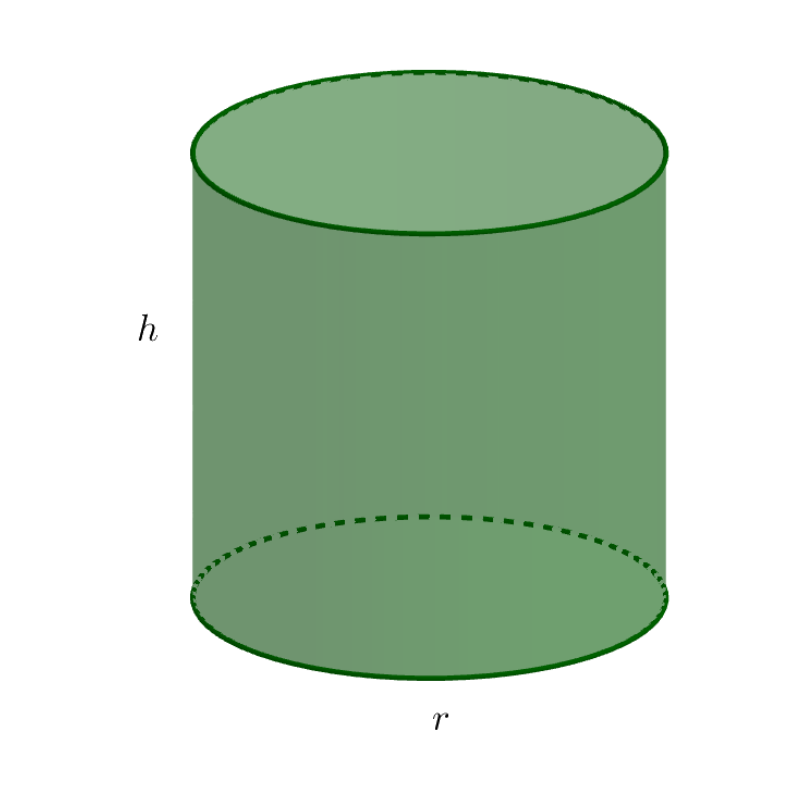
\includegraphics[width=0.8\linewidth]{mex_0024.png}
                Cilindro con altura $h=17$ cm y un radio $r=4$ cm.\\
                Volumen: \fillin[$$ u$^3$][0.4in] \\A. Lateral: \fillin[$$ u][0.4in] \\ A. Total: \fillin[$$ u$^2$][0.4in]

                % \part 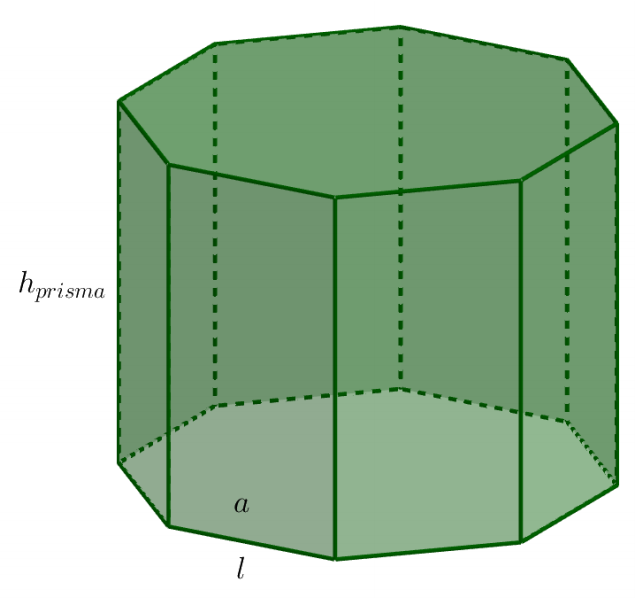
\includegraphics[width=\linewidth]{mex_0025.png}
                % Volumen: \fillin[$$ u$^3$][0.4in] \\A. Lateral: \fillin[$$ u][0.4in] \\ A. Total: \fillin[$$ u$^2$][0.4in]

                % \part 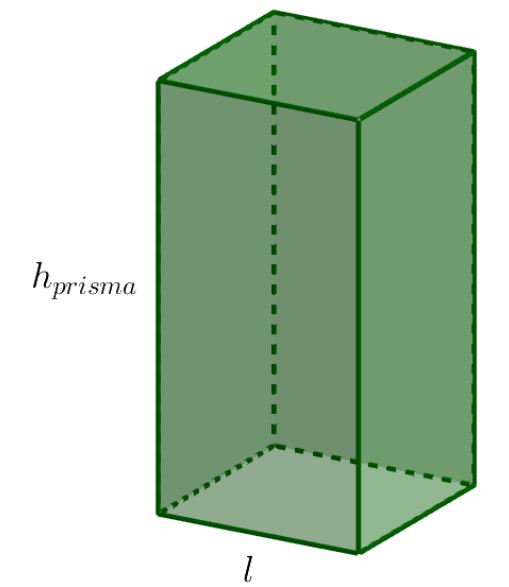
\includegraphics[width=\linewidth]{mex_0026.png}
                % Prisma cuyos lados "l" de la base miden 15 cm y la altura "h" mide 24 cm.\\
                % Volumen: \fillin[$$ u$^3$][0.4in] \\A. Lateral: \fillin[$$ u][0.4in] \\ A. Total: \fillin[$$ u$^2$][0.4in]

                \part 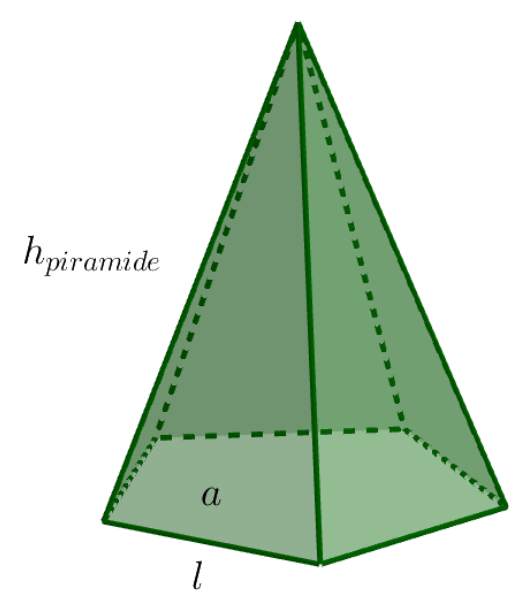
\includegraphics[width=0.8\linewidth]{mex_0027.png}
                Pirámide de 19 cm de altura cuya base es un pentágono cuyos lados "l" miden 8 cm y su apotema "a" mide 5 cm.\\
                Volumen: \fillin[$$ u$^3$][0.4in] \\A. Lateral: \fillin[$$ u][0.4in] \\ A. Total: \fillin[$$ u$^2$][0.4in]

                % \part 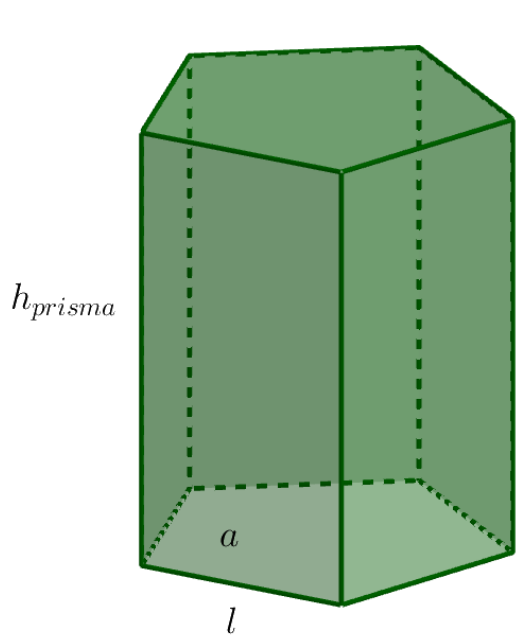
\includegraphics[width=\linewidth]{mex_0028.png}
                % Volumen: \fillin[$$ u$^3$][0.4in] \\A. Lateral: \fillin[$$ u][0.4in] \\ A. Total: \fillin[$$ u$^2$][0.4in]

                \part 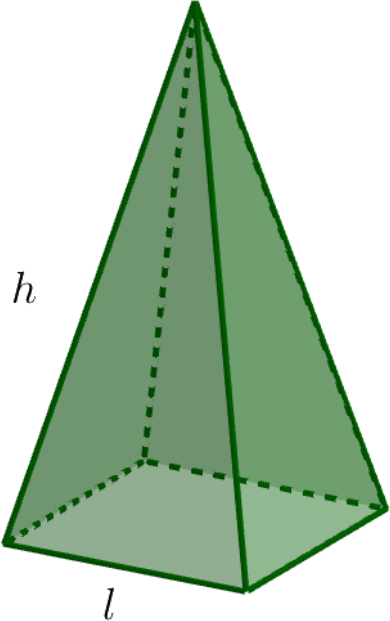
\includegraphics[width=0.8\linewidth]{mex_0029.png}
                Pirámide cuyos lados "l" de la base miden 16 cm y la altura "h" mide 27 cm.\\
                Volumen: \fillin[$$ u$^3$][0.4in] \\A. Lateral: \fillin[$$ u][0.4in] \\ A. Total: \fillin[$$ u$^2$][0.4in]

                % \part 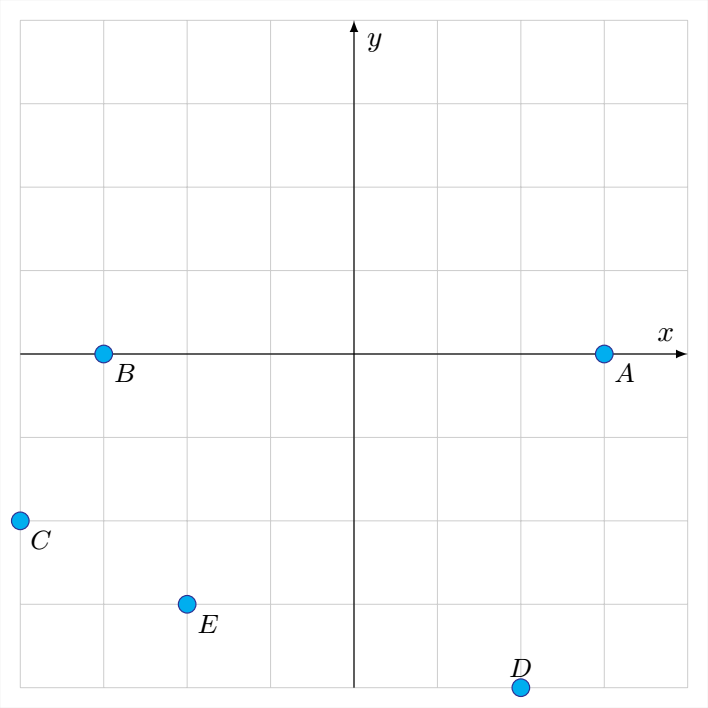
\includegraphics[width=\linewidth]{mex_0030.png}
                % Volumen: \fillin[$$ u$^3$][0.4in] \\A. Lateral: \fillin[$$ u][0.4in] \\ A. Total: \fillin[$$ u$^2$][0.4in]

            \end{parts}
        \end{multicols}
    }




    \section*{Plano cartesiano y recta}

    \subsection*{Ubicación en el plano cartesiano}
    \questionboxed[5]{ Observa la siguiente figura:

        \begin{minipage}{0.35\linewidth}
            \begin{figure}[H]
                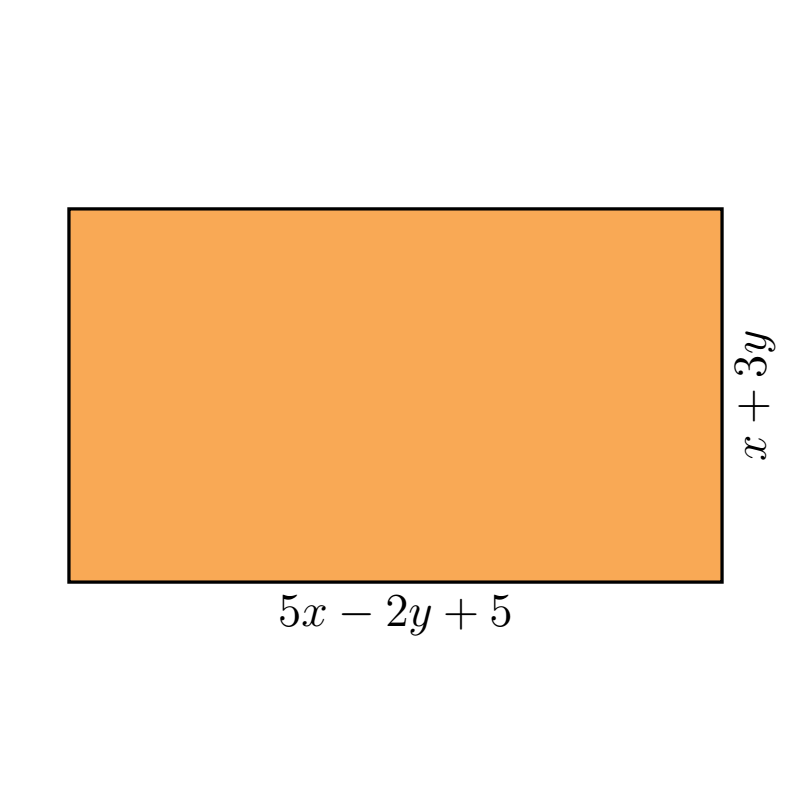
\includegraphics[width=\linewidth]{mex_0031.png}
            \end{figure}
        \end{minipage}\hfill
        \begin{minipage}{0.55\linewidth}
            \begin{parts}
                \part Escribe las coordenadas del punto A \fillin[$(,)$][0.5in]
                \part Escribe las coordenadas del punto B \fillin[$(,)$][0.5in]
                \part Escribe las coordenadas del punto C \fillin[$(,)$][0.5in]
                \part Escribe las coordenadas del punto D \fillin[$(,)$][0.5in]
                \part Escribe las coordenadas del punto E \fillin[$(,)$][0.5in]
            \end{parts}
        \end{minipage}
    }

    \questionboxed[5]{
        \begin{parts}
            \part ¿En qué cuadrante está ubicado el punto A?

            \begin{oneparchoices}
                \choice Cuadrante I
                \choice Cuadrante II
                \choice Cuadrante III
                \choice Cuadrante IV
            \end{oneparchoices}

            \part ¿En qué cuadrante está ubicado el punto B?

            \begin{oneparchoices}
                \choice Cuadrante I
                \choice Cuadrante II
                \choice Cuadrante III
                \choice Cuadrante IV
            \end{oneparchoices}

            \part ¿En qué cuadrante está ubicado el punto C?

            \begin{oneparchoices}
                \choice Cuadrante I
                \choice Cuadrante II
                \choice Cuadrante III
                \choice Cuadrante IV
            \end{oneparchoices}

            \part ¿En qué cuadrante está ubicado el punto D?

            \begin{oneparchoices}
                \choice Cuadrante I
                \choice Cuadrante II
                \choice Cuadrante III
                \choice Cuadrante IV
            \end{oneparchoices}

            \part ¿En qué cuadrante está ubicado el punto E?

            \begin{oneparchoices}
                \choice Cuadrante I
                \choice Cuadrante II
                \choice Cuadrante III
                \choice Cuadrante IV
            \end{oneparchoices}
        \end{parts}
    }

    \subsection*{Ecuación de una recta}
    \questionboxed[3]{Escribe la ecuación de las recta para dada uno de los siguientes incisos:
        \begin{parts}
            \part Escribe la ecuación de la recta que pasa por los puntos A(3,-2) y B(4,6).
            \part Escribe la ecuación de la recta que pasa por los puntos A(1,6) y B(2,1)
            \part Escribe la ecuación de la recta que pasa por los puntosA(-2,3) y B(1,0)

        \end{parts}
    }

    \subsection*{Cuadrantes en el plano cartesiano}
    \questionboxed[6]{Selecciona la respuesta correcta:
        \begin{multicols}{3}
            \begin{parts}
                \part El punto A$(0,8.24)$, ¿está ubicado sobre el eje $y$?

                \begin{oneparcheckboxes}
                    \CorrectChoice Verdadero
                    \choice Falso
                \end{oneparcheckboxes}

                \part El punto A$(0,-10)$, ¿está ubicado sobre el eje $x$?

                \begin{oneparcheckboxes}
                    \choice Verdadero
                    \CorrectChoice Falso
                \end{oneparcheckboxes}

                \part El punto A$(2,0)$, ¿está ubicado sobre el eje $y$?

                \begin{oneparcheckboxes}
                    \choice Verdadero
                    \CorrectChoice Falso
                \end{oneparcheckboxes}

                \part El punto A$(0,-5.19)$, ¿está ubicado sobre el eje $x$?

                \begin{oneparcheckboxes}
                    \choice Verdadero
                    \CorrectChoice Falso
                \end{oneparcheckboxes}

                \part El punto A$(-1.5,0)$, ¿está ubicado sobre el eje $x$?

                \begin{oneparcheckboxes}
                    \CorrectChoice Verdadero
                    \choice Falso
                \end{oneparcheckboxes}

                \part El punto A$(1,0)$, ¿está ubicado sobre el eje $x$?

                \begin{oneparcheckboxes}
                    \CorrectChoice Verdadero
                    \choice Falso
                \end{oneparcheckboxes}
            \end{parts}
        \end{multicols}
    }
    \subsection*{Pendiente y ordenada}
    \questionboxed[5]{Identifica la pendiente y ordenada de las siguientes rectas:
        \begin{parts}
            \begin{multicols}{3}
                \part $y=-2x+1$ \\[1em]
                Pendiente = \fillin[$-2$][0in] \\  Ordenada = \fillin[$1$][0in]

                \part $y=\dfrac{1}{2}x-3$ \\[1em]
                Pendiente = \fillin[$\dfrac{1}{2}$][0in]  \\ Ordenada = \fillin[$-3$][0in]

                \part $y=-3x+3$ \\[1em]
                Pendiente = \fillin[$-3$][0in] \\  Ordenada = \fillin[$3$][0in]
            \end{multicols}

            \begin{multicols}{2}
                \part 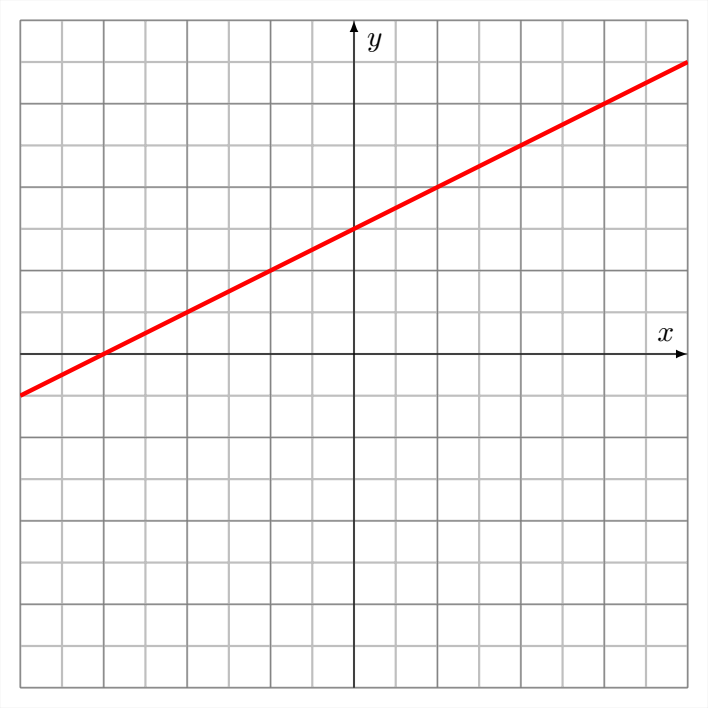
\includegraphics[width=0.8\linewidth]{mex_0047.png}\\
                Pendiente = \fillin[$-2$][0in] \qquad \qquad Ordenada = \fillin[$1$][0in]

                \part 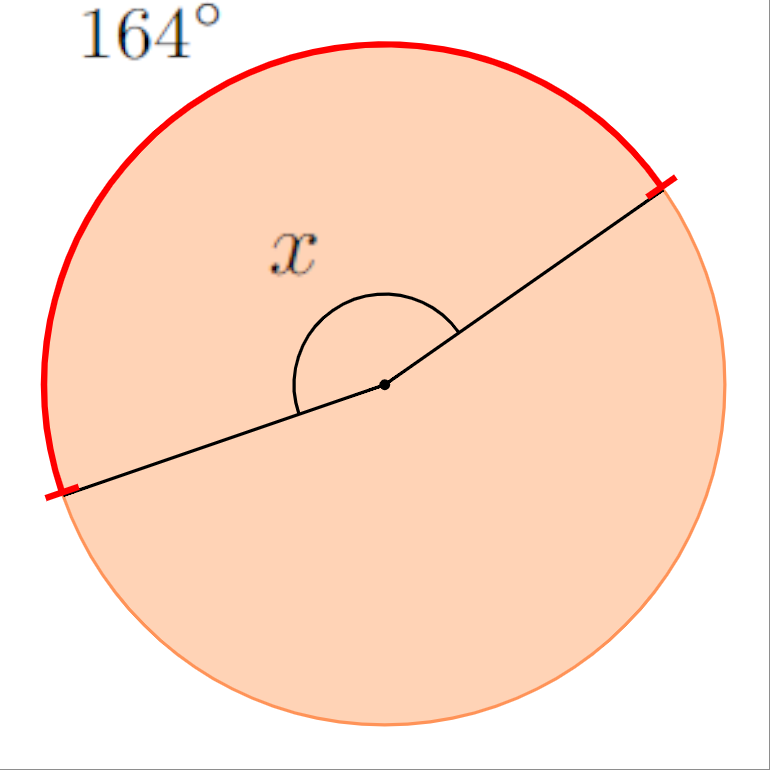
\includegraphics[width=0.8\linewidth]{mex_0051.png}\\
                Pendiente = \fillin[$-2$][0in]  \qquad \qquad Ordenada = \fillin[$1$][0in]
            \end{multicols}

        \end{parts}
    }



    \subsection*{Pendiente dados dos puntos}
    \questionboxed[7]{Calcula la pendiente en cada uno de los siguientes incisos:
        \begin{multicols}{2}

            \begin{parts}
                \part Calcula la pendiente de la recta que pasa por los puntos A(0,-3) y B(5,1).   \\[1em]
                $m=$ \fillin[$\dfrac{4}{5}$][0in]
                \part Calcula la pendiente de la recta que pasa por los puntos A(-8,6) y B(-3,8).  \\[1em]
                $m=$ \fillin[$\dfrac{2}{5}$][0in]
                \part Calcula la pendiente de la recta que pasa por los puntos A(1,1) y B(5,-3).   \\[1em]
                $m=$ \fillin[$-1$][0in]
                \part Calcula la pendiente de la recta que pasa por los puntos A(-7,-3) y B(6,10). \\[1em]
                $m=$ \fillin[$1$][0in]
                \part Calcula la pendiente de la recta que pasa por los puntos A(-7,-3) y B(-5,7). \\[1em]
                $m=$ \fillin[$5$][0in]

                \part Calcula la pendiente de la siguiente recta:\\
                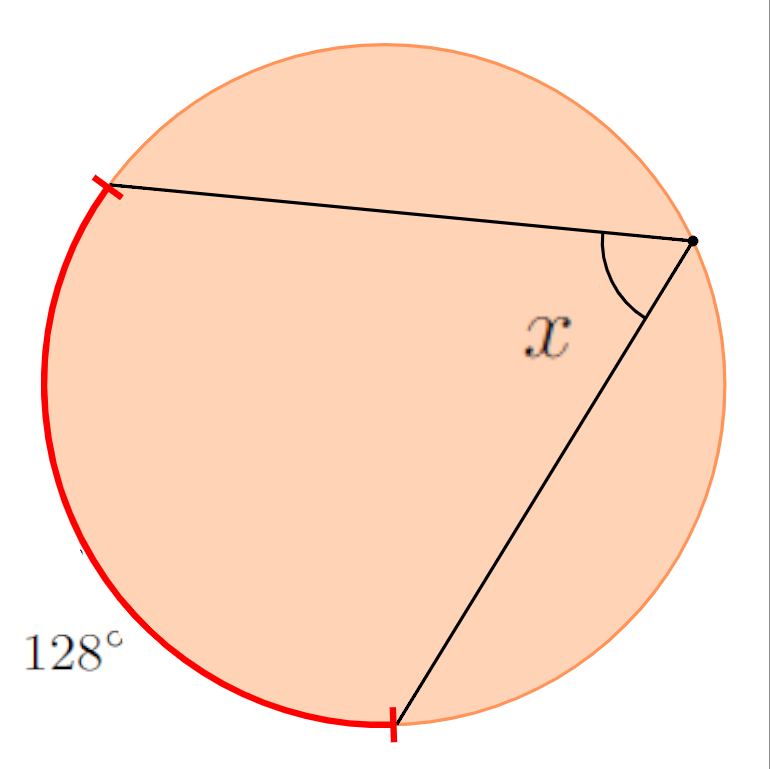
\includegraphics[width=0.8\linewidth]{mex_0050.png} $m=$ \fillin[$-1$][0in]

                \part Calcula la pendiente de la siguiente recta:\\
                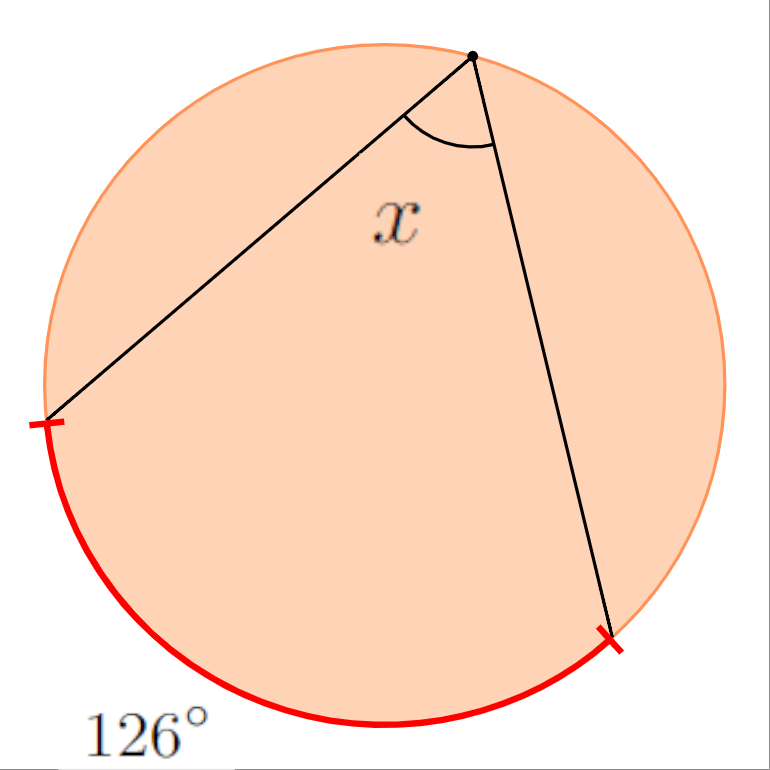
\includegraphics[width=0.8\linewidth]{mex_0048.png} $m=$ \fillin[$\dfrac{4}{5}$][0in]
            \end{parts}
        \end{multicols}
    }

    \section*{Ecuación lineal}

    \subsection*{Ecuaciones lineales}
    \questionboxed[3]{Resuelve las siguientes ecuaciones lineales
        \begin{multicols}{3}
            \begin{parts}
                % \part $2x=-30$         \fillin[$x=-15$][0in]            \\
                % \part $x-23=-36$       \fillin[$x=-13$][0in]            \\
                % \part $-4x=-6$         \fillin[$x=\dfrac{3}{2}$][0in]   \\
                % \part $6x=-36$         \fillin[$x=-6$][0in]             \\
                \part $6x-2=10$        \fillin[$x=2$][0in]
                \begin{solutionbox}{1.5cm}
                \end{solutionbox}

                % \part $12x-36=-60$     \fillin[$x=-2$][0in]           \\
                % \part $-4x+1=2x+7$     \fillin[$x=-1$][0in]           \\
                \part $9x-8=5x+4$      \fillin[$x=3$][0in]

                \begin{solutionbox}{1.5cm}
                \end{solutionbox}
                % \part $5(-3x+5)=20$    \fillin[$x=\dfrac{1}{3}$][0in] \\

                \part $32x+24=5(2x-4)$ \fillin[$x=-2$][0in]

                \begin{solutionbox}{1.5cm}
                \end{solutionbox}
            \end{parts}
        \end{multicols}
    }

    \subsection*{Lenguaje algebraico}
    \questionboxed[7]{Escribe la expresión algebraica correcta para los siguientes enunciados
        \begin{multicols}{2}
            \begin{parts}
                \part La cuarta parte de un número cualquiera.

                \begin{solutionbox}{1cm}
                    $\dfrac{x}{4}$ o $\dfrac{1}{4}x$
                \end{solutionbox}
                % \part El producto de tres números cualquiera.                \\ \fillin[$xyz$][0.5in]

                \part El cuadrado de la diferencia de dos números cualquiera.

                \begin{solutionbox}{1cm}
                    $(x-y)^2$
                \end{solutionbox}

                \part El cubo de un número cualquiera aumentado en 10.

                \begin{solutionbox}{1cm}
                    $x^3+10$
                \end{solutionbox}

                \part El cuadrado de la suma de dos números cualquiera.

                \begin{solutionbox}{1cm}
                    $(x+y)^2$
                \end{solutionbox}

                \part El recíproco de un número cualquiera.

                \begin{solutionbox}{1cm}
                    $\dfrac{1}{x}$
                \end{solutionbox}

                \part El triple de un número cualquiera.

                \begin{solutionbox}{1cm}
                    $3x$
                \end{solutionbox}

                % \part El doble del cuadrado de un número cualquiera.                       

                % \begin{solutionbox}{1cm}
                %     $2x^2$
                % \end{solutionbox}

                \part La mitad del cubo de la suma de dos números cualquiera.

                \begin{solutionbox}{1cm}
                    $\dfrac{1}{2}(x+y)^3$
                \end{solutionbox}

                \part Dos novenas partes de un número cualquiera.

                \begin{solutionbox}{1cm}
                    $\dfrac{2}{9}x$
                \end{solutionbox}

            \end{parts}
        \end{multicols}
    }


    \subsection*{Resolución de problemas}
    \questionboxed[2]{Resuelve los siguientes problemas de ecuaciones lineales
        \begin{parts}
            \part La suma de tres números consecutivos es 195. Halla estos números
            \begin{solutionbox}{2cm}
            \end{solutionbox}
            \part La suma de dos números es 215 y el mayor excede al menor en 31 unidades. ¿Cuáles son estos dos números?
            \begin{solutionbox}{2cm}
            \end{solutionbox}
        \end{parts}

    }

    \subsection*{Ecuaciones lineales con fracciones}
    \questionboxed[10]{Resuelve las siguientes ecuaciones lineales con fracciones

        \begin{multicols}{2}
            \begin{parts}
                \part $-\dfrac{1}{2}x-\dfrac{1}{4}x=\dfrac{5}{6}$

                \begin{solutionbox}{1.5cm}
                \end{solutionbox}

                \part $-\dfrac{x}{6}=\dfrac{7}{54}$
                \begin{solutionbox}{1.5cm}
                \end{solutionbox}

            \end{parts}
        \end{multicols}

    }



    \section*{Sistemas de ecuaciones}
    \questionboxed[15]{Numera correctamente los pasos para resolver un sistema de dos ecuaciones con dos inc\'ognitas por los m'etodos a continuaci\'on:
        \begin{choices}
            \choice M\'etodo de sustitución:
            \begin{itemize}
                \item[\rule{1cm}{0.2mm}] Despejar una inc\'ognita en una de las ecuaciones.
                \item[\rule{1cm}{0.2mm}] Resolver la ecuaci\'on resultante.
                \item[\rule{1cm}{0.2mm}] Sustituir el valor obtenido en la ecuaci\'on en la que aparec\'ia la inc\'ognita despejada.
                \item[\rule{1cm}{0.2mm}] Sustituir la expresi\'on de esta inc\'ognita en la otra ecuaci\'on para obtener una ecuaci\'on con una sola inc\'ognita.
                \item[\rule{1cm}{0.2mm}] Sustituir los valores en las ecuaciones originales para comprobar que son la soluci\'on.
            \end{itemize}

            \choice M\'etodo de suma-resta:
            \begin{itemize}
                \item[\rule{1cm}{0.2mm}] Resolver la ecuaci\'on resultante.
                \item[\rule{1cm}{0.2mm}] Sumar o restar las ecuaciones para eliminar una de las inc\'ognitas.
                \item[\rule{1cm}{0.2mm}] Sustituir los valores en las ecuaciones originales para comprobar que son la soluci\'on.
                \item[\rule{1cm}{0.2mm}] Multiplicar una o ambas ecuaciones por los n\'umeros necesarios para realizar la eliminaci\'on bajo la suma o resta.
                \item[\rule{1cm}{0.2mm}] Sustituir el valor obtenido en una de las ecuaciones iniciales y resolverla.
            \end{itemize}


            \choice M\'etodo de igualaci\'on:
            \begin{itemize}
                \item[\rule{1cm}{0.2mm}] Resolver la ecuaci\'on resultante.
                \item[\rule{1cm}{0.2mm}] Despejar la misma inc\'ognita en ambas ecuaciones.
                \item[\rule{1cm}{0.2mm}] Sustituir los valores en las ecuaciones originales para comprobar que son la soluci\'on.
                \item[\rule{1cm}{0.2mm}] Igualar las expresiones para obtener una ecuaci\'on con una inc\'ognita
                \item[\rule{1cm}{0.2mm}] Sustituir el valor obtenido en cualquiera de las dos expresiones en las que aparec\'ia despejada la otra inc\'ognita.
            \end{itemize}
        \end{choices}
    }

    \questionboxed[4]{Utilizando el m\'etodo de tu preferencia, encuentra el valor de $x$ y $y$ para
        cada uno de los siguientes sistemas de ecuaciones lineales:
        \begin{multicols}{2}
            \begin{parts}
                \part
                \begin{eqnarray}
                    2x-y & = & 3 \nonumber\\
                    3x-y & = & 3 \nonumber
                \end{eqnarray}

                \begin{solutionbox}{4cm}
                \end{solutionbox}

                \part
                \begin{eqnarray}
                    13x-6y & = & 22 \nonumber\\
                    x & = & y+6 \nonumber
                \end{eqnarray}

                \begin{solutionbox}{4cm}
                \end{solutionbox}
                % \vspace{4cm}
            \end{parts}
        \end{multicols}
    }
    % \subsection*{{Método de eliminación}
    % \subsection*{{Método de sustitución e igualación}
    \subsection*{Sistema de ecuaciones 3x3}
    \questionboxed[5]{Resuelve el siguiente sistema de ecuaciones lineales:

        \begin{align*}
            x + 2y +3z  & = 12 \\
            x - 3y +4z  & = 27 \\
            -x +  y +2z & = 7
        \end{align*}

        \begin{solutionbox}{8cm}
        \end{solutionbox}
    }
    \subsection*{Sistema de ecuaciones con fracciones}
    \questionboxed[5]{Resuelve el siguiente sistema de ecuaciones lineales con fracciones:
        \begin{align*}
            12x + 5y                      & = -6  \\
            \dfrac{5}{3}x - \dfrac{7}{6}y & = -12
        \end{align*}
        \begin{solutionbox}{8cm}
        \end{solutionbox}
    }

    % \subsection*{{Resolución de problemas}
\end{questions}
\end{document}